%%%%%%%%%%%%%%%%%%%%%%%%%%%%%%%%%%%%%%%%%%%%%%%%%%%%%%%%%%%%%%
%%%                                                        %%%
%%%        IMPORTANT - DO NOT ADD EXERCISES HERE           %%%
%%%                                                        %%%
%%%    ALL EXERCISES MUST FIRST GO TO SOLUTION MANUAL,     %%%
%%%       THEN STRIPPED OFF SOLUTIONS AND GO HERE          %%%
%%%                                                        %%%
%%%%%%%%%%%%%%%%%%%%%%%%%%%%%%%%%%%%%%%%%%%%%%%%%%%%%%%%%%%%%%

%%%%%%%%%%%%%%%%%%%%%%%%%%%%%%%%%%%%%%%%%%%%%%%%%%%%%%%%%%%%%%%%%%%%%%%%%%%%

\section{Introduction}

All exercises from this textbook can be cloned in NCLab through the {\em Project
$\rightarrow$ Clone} menu. Solution Manual is available in NCLab starting with Basic 
Version. To warm up, in this section we will experiment with the {\tt print} 
command.

%%%%%%%%%%%%%%%%%%%%%%%%%%%%%%%%%%%%%%%%%%%%%%%%%%%%%%%%%%%%%%%%%%%%%%%%%%%%

\subsection{Python is fun}

Write a program that prints the phrase "Python is fun" 
\begin{enumerate}
\item As separate words on three lines, one word per line, aligned to the left.
\item On one line.
\item On one line, inside a box made up of the characters '=' and '|'.
\end{enumerate}

%%%%%%%%%%%%%%%%%%%%%%%%%%%%%%%%%%%%%%%%%%%%%%%%%%%%%%%%%%%%%%%%%%%%%%%%%%%%

\subsection{Big word}

Write a program that prints the word "Python" in large block 
letters as shown below:

\begin{bluecode}
XXXXX Y   X XXXXX X   X XXXXX X   X
X   X Y   X   X   X   X X   X XX  X
XXXXX XXXXX   X   XXXXX X   X X X X
X         X   X   X   X X   X X  XX
X     XXXXX   X   X   X XXXXX X   X
\end{bluecode}

%%%%%%%%%%%%%%%%%%%%%%%%%%%%%%%%%%%%%%%%%%%%%%%%%%%%%%%%%%%%%%%%%%%%%%%%%%%%

\subsection{Military exercise}

Save the program from the previous exercise under the name 
"George Smith" and adjust it to print the name of a famous American
general who during the World War 2 commanded U.S. Army Troops
in North Africa and Europe. 

%%%%%%%%%%%%%%%%%%%%%%%%%%%%%%%%%%%%%%%%%%%%%%%%%%%%%%%%%%%%%%%%%%%%%%%%%%%%
%%%%%%%%%%%%%%%%%%%%%%%%%%%%%%%%%%%%%%%%%%%%%%%%%%%%%%%%%%%%%%%%%%%%%%%%%%%%

\section{Using Python as a Calculator}

In this section we will practice using Python's interactive shell for simple 
as well as advanced arithmetic operations.

%%%%%%%%%%%%%%%%%%%%%%%%%%%%%%%%%%%%%%%%%%%%%%%%%%%%%%%%%%%%%%%%%%%%%%%%%%%%

\subsection{Grocery shopping}

Today you went grocery shopping and you bought:
\begin{enumerate}
\item Two cans of an energy drink for \$1.56 a piece.
\item Three bottles of milk \$2.34 a piece.
\item Four French baguettes \$3.41 a piece.
\item Five packs of chewing gum \$0.99 a piece.
\end{enumerate}
Tax in the amount of 8\% applies to items 1 and 4.
Calculate the total cost of your purchase!

%%%%%%%%%%%%%%%%%%%%%%%%%%%%%%%%%%%%%%%%%%%%%%%%%%%%%%%%%%%%%%%%%%%%%%%%%%%%

\subsection{Oil change}

You decided to do oil change today since your favorite 
place offers 20\% off. The oil costs \$45 plus 8\% tax. 
The work is 25 dollars. Do not forget to take the 20\% off the 
total. How much will you pay for this oil change? 

%%%%%%%%%%%%%%%%%%%%%%%%%%%%%%%%%%%%%%%%%%%%%%%%%%%%%%%%%%%%%%%%%%%%%%%%%%%%

\subsection{Age average}

You go on a hike with a group of people of different 
ages. Your are (say) 15 years old. Two other people 
are 21 years old, one is 35, one is 42, and one is 55.
Calculate the average age in the group!

%%%%%%%%%%%%%%%%%%%%%%%%%%%%%%%%%%%%%%%%%%%%%%%%%%%%%%%%%%%%%%%%%%%%%%%%%%%%

\subsection{Saving for a bike}

Your savings account grows at a rate of 3\% annually. Three years ago you 
started by inserting \$1,250 into the account. One year later 
you added another \$500, and a year ago you withdrew \$300. 
How much money is in your savings account now?

%%%%%%%%%%%%%%%%%%%%%%%%%%%%%%%%%%%%%%%%%%%%%%%%%%%%%%%%%%%%%%%%%%%%%%%%%%%%

\subsection{Growing town}

For the last 20 years, the population of a city has been growing 
steadily by 5\% per year, and 20 years ago it had 10,000 inhabitants.
How many people live in the city now? Round the result to be an 
integer number.

%%%%%%%%%%%%%%%%%%%%%%%%%%%%%%%%%%%%%%%%%%%%%%%%%%%%%%%%%%%%%%%%%%%%%%%%%%%%

\subsection{Coffee maker}

How many cups of coffee will you be able to make from a one kilogram
pack when 11 grams are needed for one cup? How many grams will be 
left?

%%%%%%%%%%%%%%%%%%%%%%%%%%%%%%%%%%%%%%%%%%%%%%%%%%%%%%%%%%%%%%%%%%%%%%%%%%%%

\subsection{Gardening}

You are buying plants for an orchard restoration project.
How many plants can you purchase with \$250 if the price 
of one is \$17? How much money will you have left?  

%%%%%%%%%%%%%%%%%%%%%%%%%%%%%%%%%%%%%%%%%%%%%%%%%%%%%%%%%%%%%%%%%%%%%%%%%%%%

\subsection{Setting tiles}

You are setting tiles in a room of rectangular shape whose edges measure 19 and 27 feet. 
The tiles are 1.25 $\times$ 1.25 foot squares and they will be aligned with the walls
in the simplest possible pattern. You need 
to leave a quarter inch between the tiles for grout. How many whole tiles are you going to use?
Hint: integer part of a real number {\tt x} is obtained via {\tt int(x)}.

%%%%%%%%%%%%%%%%%%%%%%%%%%%%%%%%%%%%%%%%%%%%%%%%%%%%%%%%%%%%%%%%%%%%%%%%%%%%

\subsection{Submerged soccer ball}

The famous Archimedes' law states that the upward buoyant force exerted on a body 
immersed in a fluid is equal to the weight of the fluid the body displaces.
Imagine that you submerge a soccer ball -- neglecting its own weight, this 
is the force that you need to employ to keep it under water! Let's calculate 
this force, assuming that the ball is a perfect sphere of diameter 22 cm.
The density of water is 1000 kg/m${^3}$ and gravitational acceleration 
is 9.81 ms${^{-2}}$. 

%%%%%%%%%%%%%%%%%%%%%%%%%%%%%%%%%%%%%%%%%%%%%%%%%%%%%%%%%%%%%%%%%%%%%%%%%%%%

\subsection{Fastest runner}

Arguably, the fastest human runner in history achieved a speed of 12.1 m/s. 
Calculate how much time in seconds such a runner would need to cross a football 
field at this speed, running diagonally from one corner to the opposite one. 
The measures of a football field are 109.7 m and 48.8 m. 

%%%%%%%%%%%%%%%%%%%%%%%%%%%%%%%%%%%%%%%%%%%%%%%%%%%%%%%%%%%%%%%%%%%%%%%%%%%%

\subsection{Triangle area}

Heron's formula is a famous formula that allows you to calculate the area $S$ of a 
general triangle knowing its edge lengths $a$, $b$ and $c$:

$$
S = \sqrt{p(p-a)(p-b)(p-c)}
$$
where $p = (a + b + c)/2$. Calculate in this way the area of a triangle with sides 
2.5 m, 3.7 m and 4.1 m!

%%%%%%%%%%%%%%%%%%%%%%%%%%%%%%%%%%%%%%%%%%%%%%%%%%%%%%%%%%%%%%%%%%%%%%%%%%%%

\subsection{Math functions}

Calculate the following values:
$$
a = e^5,
$$
$$
b = \sin(\pi/3),
$$
$$
c = \cos(\pi/4),
$$
$$
d = \log(10).
$$
Here log is the natural logarithm.

%%%%%%%%%%%%%%%%%%%%%%%%%%%%%%%%%%%%%%%%%%%%%%%%%%%%%%%%%%%%%%%%%%%%%%%%%%%%

\subsection{Random numbers}

Random numbers are generated using the function {\tt random()} from the {\tt random}
library. This function returns a random real number between 0 and 1. 
Use this function to generate a random integer between 
10 and 20!

%%%%%%%%%%%%%%%%%%%%%%%%%%%%%%%%%%%%%%%%%%%%%%%%%%%%%%%%%%%%%%%%%%%%%%%%%%%%

\subsection{Greatest common divisor}

Python has a built-in function {\tt gcd()} to calculate the greatest common divisor (GCD)
of two integers. It is imported via {\tt from fractions import gcd}. Use 
the function to find the GCD of 1554 and 2331!

%%%%%%%%%%%%%%%%%%%%%%%%%%%%%%%%%%%%%%%%%%%%%%%%%%%%%%%%%%%%%%%%%%%%%%%%%%%%

\subsection{Fractions}

Python makes operations with fractions very simple via the {\tt Fraction}
function that is imported from the {\tt fractions} library. Then 
a fraction {\tt 1/3} is defined simply as {\tt Fraction(1, 3)} and so on. Fractions
can be used with the same operations as numbers, and the result of such 
an operation is a {\tt Fraction}. Now to your task: Use Fractions to 
calculate
$$
\frac{1}{2} - \frac{1}{3} + \frac{1}{4} - \frac{1}{5} + \frac{1}{6} - \frac{1}{7}.
$$

%%%%%%%%%%%%%%%%%%%%%%%%%%%%%%%%%%%%%%%%%%%%%%%%%%%%%%%%%%%%%%%%%%%%%%%%%%%%
%%%%%%%%%%%%%%%%%%%%%%%%%%%%%%%%%%%%%%%%%%%%%%%%%%%%%%%%%%%%%%%%%%%%%%%%%%%%

\section{Functions}

In this section we will practise defining and using custom functions.

\subsection{Circle}

Write a Python function {\tt circle(R)} that accept an arbitrary radius {\tt R}
as argument, and returns the area and the perimeter of a circle with radius {\tt R}.

%%%%%%%%%%%%%%%%%%%%%%%%%%%%%%%%%%%%%%%%%%%%%%%%%%%%%%%%%%%%%%%%%%%%%%%%%%%%

\subsection{Square}

Write a Python function {\tt squarearea(a)} that returns the area of a square whose 
edge is {\tt a} cm long. You know that most of the time the edge length wil be 1 cm,
so make this function callable without any arguments.

%%%%%%%%%%%%%%%%%%%%%%%%%%%%%%%%%%%%%%%%%%%%%%%%%%%%%%%%%%%%%%%%%%%%%%%%%%%%

\subsection{Rectangle}

Write a Python function {\tt rectanglearea(a, b)} that returns the area of a rectangle 
whose edges are $a$ and $b$ cm long. You know that most of the time one of the edges 
will measure 3 cm, so make the function callable with only one argument.

%%%%%%%%%%%%%%%%%%%%%%%%%%%%%%%%%%%%%%%%%%%%%%%%%%%%%%%%%%%%%%%%%%%%%%%%%%%%

\subsection{Sales prediction}

The East Coast sales division of a company usually generates $P$
percent of total sales each year. Write a function {\tt sales\_prediction(P, S)} to predict how much 
the East Coast division will generate if the company has $S$ dollars in sales the next year. 
Use your function with the numbers $P = 62\ \%$ and $S = 4.6$ million dollars. 

%%%%%%%%%%%%%%%%%%%%%%%%%%%%%%%%%%%%%%%%%%%%%%%%%%%%%%%%%%%%%%%%%%%%%%%%%%%%

\subsection{Sales tax}

Write a function {\tt sales\_tax(P, ST, CT)} that calculates the total sales tax on a $P$ dollars purchase. 
Assume the state sales tax is $ST$ percent, and the county sales tax is $CT$ percent. Use the
function with the following numbers: $P = 52$ dollars, $ST = 5 \ \%$, $CT = 2 \ \%$.

%%%%%%%%%%%%%%%%%%%%%%%%%%%%%%%%%%%%%%%%%%%%%%%%%%%%%%%%%%%%%%%%%%%%%%%%%%%%

\subsection{Restaurant bill}

Write a function {\tt restaurant\_bill(M, P, T)} 
that computes the tax and tip on a restaurant bill for a patron with 
$M$ dollars meal charge. The tax is $P$ percent of the meal cost. 
The tip is $T$ percent of the total after 
adding the tax. Your function should return the tax amount, tip amount, and the total bill. 
Use your function with the numbers $M = 44.50$ dollars, $P = 6.75 \ \%$ and $T = 15 \ \%$. 

%%%%%%%%%%%%%%%%%%%%%%%%%%%%%%%%%%%%%%%%%%%%%%%%%%%%%%%%%%%%%%%%%%%%%%%%%%%%

\subsection{Gas consumption conversion I (EU to US)}

In Europe, gas consumption of a car is reported in liters per 100 kilometers. In the U.S. 
it is reported in miles per gallon. Write a function {\tt conversion\_eu\_to\_us(C)} that converts a given European 
gas consumption $C$ into the U.S. scale. One mile is 1.609344 kilometers, and one gallon is 3.78541178 liters. 

%%%%%%%%%%%%%%%%%%%%%%%%%%%%%%%%%%%%%%%%%%%%%%%%%%%%%%%%%%%%%%%%%%%%%%%%%%%%

\subsection{Gas consumption conversion II (US to EU)}

In Europe, gas consumption of a car is reported in liters per 100 kilometers. In the U.S. 
it is reported in miles per gallon. Write a function {\tt conversion\_us\_to\_eu(C)} that converts a given U.S. gas 
consumption $C$ into the European scale. One mile is 1.609344 kilometers, and one gallon is 3.78541178 liters. 

%%%%%%%%%%%%%%%%%%%%%%%%%%%%%%%%%%%%%%%%%%%%%%%%%%%%%%%%%%%%%%%%%%%%%%%%%%%%

\subsection{Distance per tank of gas}

A car with a $G$ gallon gas tank averages $A$ miles per gallon 
when driven in town and 
$B$ miles per gallon when driven on the highway. Write a function {\tt distance(G, A, B)} 
that returns the distance the car can travel on one tank of gas when driven in town and when driven on the highway. 
Use your function with $G = 20$ gallons, $A = 21.5$ miles per gallon, $B = 26.8$ miles per gallon. 

%%%%%%%%%%%%%%%%%%%%%%%%%%%%%%%%%%%%%%%%%%%%%%%%%%%%%%%%%%%%%%%%%%%%%%%%%%%%

\subsection{Circuit board price}

An electronics company sells circuit boards at a $P$ percent profit. 
Write a function {\tt circuit\_ board\_price(P, D)} 
that calculates the selling price of a circuit board that costs them $D$ dollars to
produce. Use your function with $P = 40\ \%$ and $D = 12.67$ dollars.

%%%%%%%%%%%%%%%%%%%%%%%%%%%%%%%%%%%%%%%%%%%%%%%%%%%%%%%%%%%%%%%%%%%%%%%%%%%%

\subsection{Gross pay}

A particular employee earns $E$ dollars annually. Write a function 
{\tt gross\_pay(E)} that determines and prints what the amount of his gross pay will be for each pay period 
if he is paid twice a month (24 pay checks per year) and if he is paid bi-weekly (26 checks per 
year). Use your function with $E = 32,500$ dollars.

%%%%%%%%%%%%%%%%%%%%%%%%%%%%%%%%%%%%%%%%%%%%%%%%%%%%%%%%%%%%%%%%%%%%%%%%%%%%

\subsection{Stock gain}

Kathryn bought $N$ shares of stock at a price of $A$ dollars per share. One year later she 
sold them for $B$ dollars per share. Write a function {\tt stock\_gain(N, A, B)} that calculates and 
displays the following:
\begin{itemize}
\item The total amount paid for the stock.
\item The total amount received from selling the stock.
\item The total amount of money she gained.
\end{itemize}
Use your function with the values $N = 600$, $A = 21.77$ dollars and $B = 26.44$ dollars.

%%%%%%%%%%%%%%%%%%%%%%%%%%%%%%%%%%%%%%%%%%%%%%%%%%%%%%%%%%%%%%%%%%%%%%%%%%%%

\subsection{Temperature conversion I (Fahrenheit to Celsius)}

Write a function {\tt temperature\_conversion\_FC(F)} that converts 
temperature {\tt F} from Fahrenheit to Celsius and returns the
result. The corresponding formula is 
$$
C = \frac{5}{9}(F - 32).
$$

%%%%%%%%%%%%%%%%%%%%%%%%%%%%%%%%%%%%%%%%%%%%%%%%%%%%%%%%%%%%%%%%%%%%%%%%%%%%

\subsection{Temperature conversion II (Celsius to Fahrenheit)}

Write a function {\tt temperature\_conversion\_CF(C)} that converts 
temperature {\tt C} from Celsius to Fahrenheit and returns the
result. The corresponding formula is 
$$
F = \frac{9}{5}C + 32.
$$

%%%%%%%%%%%%%%%%%%%%%%%%%%%%%%%%%%%%%%%%%%%%%%%%%%%%%%%%%%%%%%%%%%%%%%%%%%%%

\subsection{Time in seconds}

Write a function {\tt time\_in\_seconds(H, M, S)} where H, M, S are
integer numbers representing hours, minutes and seconds. Convert this 
time period into seconds, and return it. 

%%%%%%%%%%%%%%%%%%%%%%%%%%%%%%%%%%%%%%%%%%%%%%%%%%%%%%%%%%%%%%%%%%%%%%%%%%%%

\subsection{Time in hours}

Write a function {\tt time\_in\_hours(H, M)} where H, M are
integer numbers representing hours and minutes. Convert this 
time period into hours and return it. For example, {\tt time\_in\_hours(1, 30)}
will return {\tt 1.5}.

%%%%%%%%%%%%%%%%%%%%%%%%%%%%%%%%%%%%%%%%%%%%%%%%%%%%%%%%%%%%%%%%%%%%%%%%%%%%

\subsection{Time last time}

Write a function {\tt time\_conversion(T)} that takes 
a period of time {\tt T} in seconds (an integer number), and converts it to 
hours, minutes and seconds. It should return the corresponding 
three values H, M, S. The number H should be an integer, and both S 
and M should be integers between 0 and 59.

%%%%%%%%%%%%%%%%%%%%%%%%%%%%%%%%%%%%%%%%%%%%%%%%%%%%%%%%%%%%%%%%%%%%%%%%%%%%

\subsection{Distance}

Write a function {\tt distance(x1, y1, x2, y2)} that calculates and 
returns the distance $d$ of two points $(x_1, y_1)$ and $(x_2, y_2)$
using the formula 
$$
d = \sqrt{(x_2 - x_1)^2 + (y_2 - y_1)^2}.
$$ 

%%%%%%%%%%%%%%%%%%%%%%%%%%%%%%%%%%%%%%%%%%%%%%%%%%%%%%%%%%%%%%%%%%%%%%%%%%%%

\subsection{Angle conversion}

Write a function {\tt angle\_conversion(A)} that converts the angle A
from degrees to radians and returns the result. Use the fact that $\pi$
radians equals to 180 degrees. In order to work with {\tt pi}, you need to 
import it from Numpy first. Hence, begin your program with the line 
"{\tt from numpy import pi}".

%%%%%%%%%%%%%%%%%%%%%%%%%%%%%%%%%%%%%%%%%%%%%%%%%%%%%%%%%%%%%%%%%%%%%%%%%%%%

\subsection{Length conversion}

Write a function {\tt length\_conversion(Y, F, I)} that converts a length given
in terms of yards, feet and inches into meters. Return the result. Recall 
that one yard is 0.9144 meters, there are three feet in a yard, and 
12 inches per foot.

%%%%%%%%%%%%%%%%%%%%%%%%%%%%%%%%%%%%%%%%%%%%%%%%%%%%%%%%%%%%%%%%%%%%%%%%%%%%

\subsection{Area conversion}

Write a function {\tt area\_conversion(SF)} that converts an apartment 
area from square feet SF to square meters. Return the result. 

%%%%%%%%%%%%%%%%%%%%%%%%%%%%%%%%%%%%%%%%%%%%%%%%%%%%%%%%%%%%%%%%%%%%%%%%%%%%

\subsection{Digital storage conversion}

Write a function {\tt memory\_conversion(GB, MB, KB, B)} that converts a digital storage 
size consisting of GB gigabytes, MB megabytes, KB kilobytes, and 
B bytes to bytes. Return the result. Recall that one kilobyte 
equals to 1024 bytes, one megabyte equals to 1024 kilobytes, and 
one gigabyte is the same as 1024 megabytes.

%%%%%%%%%%%%%%%%%%%%%%%%%%%%%%%%%%%%%%%%%%%%%%%%%%%%%%%%%%%%%%%%%%%%%%%%%%%%

\subsection{Savings account}

Write a Python function {\tt savings(amount, p, num\_years)} that calculates
how much money will be in your savings account after {\tt num\_years} with 
an initial amount {\tt amount}, if every year the amount increases by {\tt p}
percent.

%%%%%%%%%%%%%%%%%%%%%%%%%%%%%%%%%%%%%%%%%%%%%%%%%%%%%%%%%%%%%%%%%%%%%%%%%%%%
%%%%%%%%%%%%%%%%%%%%%%%%%%%%%%%%%%%%%%%%%%%%%%%%%%%%%%%%%%%%%%%%%%%%%%%%%%%%

\section{Colors and plotting}

In this section we will practice plotting of various objects including polygons, 
function graphs, 2D and 3D curves, surfaces, and even pie and bar charts. 

%%%%%%%%%%%%%%%%%%%%%%%%%%%%%%%%%%%%%%%%%%%%%%%%%%%%%%%%%%%%%%%%%%%%%%%%%%%%

\subsection{Polygon}

Write a Python function {\tt polygon(R, n)} that returns two arrays {\tt x} and {\tt y}.
These arrays will contain the $x$ and $y$ coordinates of the vertices of a polygon 
with $n$ equally-long edges, that is inscribed into a circle of 
center $[0, 0]$ and radius $R > 0$. Here {\tt n > 2} is an integer number 
and {\tt R > 0} is a real number. The polygon should be oriented counter clock-wise
and the first vertex should be $[R, 0]$.
Use this function to plot a sample
polygon with parameters {\tt R = 2}, {\tt n = 6}. Make sure that axes are scaled equally.

%%%%%%%%%%%%%%%%%%%%%%%%%%%%%%%%%%%%%%%%%%%%%%%%%%%%%%%%%%%%%%%%%%%%%%%%%%%%

\subsection{Custom plotting function}

Consider an arbitrary Python function {\tt f(x)} that for a real number 
{\tt x} returns a real value. For example, such a function could be 
$f(x) = e^{-x}$:

\begin{Verbatim}[commandchars=\\\{\}]
\PY{k}{def} \PY{n+nf}{f}(x):
    \PY{k}{return} exp(-x)
\end{Verbatim}
Write a Python function {\tt plotfun(a, b, f, n)} that will return two
arrays {\tt xpts} and {\tt ypts}. The former will contain x-coordinates of 
{\tt n}-point linear subdivision of the interval {\tt [a, b]}, the latter will
contain the corresponding function values. Use the function {\tt plotfun} to
plot the graph of the function {\tt f(x)} defined above, in the interval $[-1, 1]$.
Axes should be scaled equally.

%%%%%%%%%%%%%%%%%%%%%%%%%%%%%%%%%%%%%%%%%%%%%%%%%%%%%%%%%%%%%%%%%%%%%%%%%%%%

\subsection{Planar curve}

Consider two arbitrary Python functions {\tt f(t)} and {\tt g(t)} that 
for a real number {\tt t} in the interval $[0, 1]$ return a real value. 
For example, such functions could be $f(t) = t^2 \cos(10 \pi t)$ and 
$g(t) = t^2 \sin(10 \pi t)$:

\begin{Verbatim}[commandchars=\\\{\}]
\PY{k}{def} \PY{n+nf}{f}\PY{p}{(}\PY{n}{t}\PY{p}{)}\PY{p}{:}
    \PY{k}{return} \PY{n}{cos}\PY{p}{(}\PY{l+m+mi}{2}\PY{o}{*}\PY{n}{pi}\PY{o}{*}\PY{n}{t}\PY{p}{)}

\PY{k}{def} \PY{n+nf}{g}\PY{p}{(}\PY{n}{t}\PY{p}{)}\PY{p}{:}
    \PY{k}{return} \PY{n}{sin}\PY{p}{(}\PY{l+m+mi}{2}\PY{o}{*}\PY{n}{pi}\PY{o}{*}\PY{n}{t}\PY{p}{)}
\end{Verbatim}
Write a Python function {\tt planarcurve(f, g, n)} that returns two
arrays {\tt xpts} and {\tt ypts}. These arrays will contain 'x' and 'y' coordinates of 
{\tt n} points lying on the planar curve $[f(t), g(t)]$. These points 
correspond to a linear subdivision of the parameterization interval 
$[0, 1]$ with {\tt n} points. Use the function {\tt planarcurve} to
plot the curve corresponding to the functions {\tt f(t)} and {\tt g(t)} 
defined above. Axes should be scaled equally.

%%%%%%%%%%%%%%%%%%%%%%%%%%%%%%%%%%%%%%%%%%%%%%%%%%%%%%%%%%%%%%%%%%%%%%%%%%%%

\subsection{Random triangle}

The function {\tt random()} from the {\tt random} library returns a random number between 0 and 1.  
Write a Python function {\tt tria(a, b, c, d)} that returns six numbers x1, y1, x2, y2, x3, y3. These numbers 
represent vertices [x1, y1], [x2, y2], [x3, y3] of a random triangle that lies in the rectangle (a, b)x(c, d). 
Plot the triangle. Make sure that axes are scaled equally.

%%%%%%%%%%%%%%%%%%%%%%%%%%%%%%%%%%%%%%%%%%%%%%%%%%%%%%%%%%%%%%%%%%%%%%%%%%%%

\subsection{Wireframe plot}

Write Python function {\tt wireframeplot(f, x1, x2, y1, y2, nx=30, ny=30)} where {\tt f(x, y)} is a real function 
of two variables, {\tt (x1, x2)x(y1, y2)} is the plotting rectangle, and {\tt nx}, {\tt ny} are plotting 
subdivisions in the $x$ and $y$ axial directions. Test it on the function 

$$
f(x, y) = e^{-x^2 - y^2}
$$
in the square $(-3, 3)\times (-3, 3)$.

%%%%%%%%%%%%%%%%%%%%%%%%%%%%%%%%%%%%%%%%%%%%%%%%%%%%%%%%%%%%%%%%%%%%%%%%%%%%

\subsection{Solid surface plot}

Write Python function {\tt solidsurfaceplot(f, x1, x2, y1, y2, nx=30, ny=30)} where {\tt f(x, y)} is a real function 
of two variables, {\tt (x1, x2)x(y1, y2)} is the plotting rectangle, and {\tt nx}, {\tt ny} are plotting 
subdivisions in the $x$ and $y$ axial directions. Test it on the function 
$$
f(x, y) = 5 - (x^2 + y^2)
$$
in the square $(-2, 2)\times (-2, 2)$.

%%%%%%%%%%%%%%%%%%%%%%%%%%%%%%%%%%%%%%%%%%%%%%%%%%%%%%%%%%%%%%%%%%%%%%%%%%%%

\subsection{Contour plot}

Write Python function {\tt contourplot(f, x1, x2, y1, y2, num\_contours, 
nx =30, ny=30)} where {\tt f(x, y)} is a real function 
of two variables, {\tt (x1, x2)x(y1, y2)} is the plotting rectangle, {\tt num\_contours}
is the number of contours to be displayed, and {\tt nx}, {\tt ny} are plotting 
subdivisions in the $x$ and $y$ axial directions. Display contour plot of the function 
$$
f(x, y) = xy 
$$
in the square $(-1, 1)\times (-1, 1)$ with 30 contours.

%%%%%%%%%%%%%%%%%%%%%%%%%%%%%%%%%%%%%%%%%%%%%%%%%%%%%%%%%%%%%%%%%%%%%%%%%%%%

\subsection{WebGL plot}

Solve this exercise only if WebGL works on your 
computer (WebGL Tester can be found on NCLab 
front page). Write Python function webglplot(f, x1, x2, y1, y2, nx=30, ny=30) where 
f(x, y) is a real function of two variables, (x1, x2)x(y1, y2) is the plotting 
rectangle, and nx, ny are plotting subdivisions in the x and y axial directions. 
Test it on the function

$$
f(x, y) = e^{-x^2 - y^2}
$$
in the square $(-2, 2)\times (-2, 2)$.

%%%%%%%%%%%%%%%%%%%%%%%%%%%%%%%%%%%%%%%%%%%%%%%%%%%%%%%%%%%%%%%%%%%%%%%%%%%%

\subsection{Pie chart plot}

A family spends each month $25 \%$ of their budget on clothing,
$20\%$ on food, $10\%$ on car payments, $20 \%$ on mortgage,
$5 \%$ on utilities, and they save $20 \%$. Plot a pie chart 
representing their spendings, and highlight the savings part via 
the {\tt explode} function.

%%%%%%%%%%%%%%%%%%%%%%%%%%%%%%%%%%%%%%%%%%%%%%%%%%%%%%%%%%%%%%%%%%%%%%%%%%%%
%%%%%%%%%%%%%%%%%%%%%%%%%%%%%%%%%%%%%%%%%%%%%%%%%%%%%%%%%%%%%%%%%%%%%%%%%%%%

\section{Variables}

In this section we reinforce our understanding of local and global variables.

%%%%%%%%%%%%%%%%%%%%%%%%%%%%%%%%%%%%%%%%%%%%%%%%%%%%%%%%%%%%%%%%%%%%%%%%%%%%

\subsection{Arithmetic sequence}

{\em Arithmetic sequence} is a progression of $n$ numbers $a_1$, $a_2$, $\ldots$, $a_n$
that increase by the same difference $d$. For example, 
$$
5, 7, 9, 11, 13, 15, 17
$$
is an arithmetic sequence with $n = 7$, $a_1 = 5$ and $d = 2$. It holds
$$
a_n = a_1 + (n-1)d.
$$
There is a well known formula for the sum of such a sequence:
$$
S = \frac{n}{2}(a_1 + a_n).
$$
And now the exercise: Write a function {\tt summation\_arithmetic(n, a1, d)} that takes arbitrary 
values of $n$, $a_1$ and $d$ as arguments, and calculates and returns the sum
of the corresponding arithmetic sequence!

%%%%%%%%%%%%%%%%%%%%%%%%%%%%%%%%%%%%%%%%%%%%%%%%%%%%%%%%%%%%%%%%%%%%%%%%%%%%

\subsection{Geometric sequence}

{\em Geometric sequence} is a progression of $n$ numbers $a_1$, $a_2$, $\ldots$, $a_n$
where the next number is calculated by multiplying the last one with a quotient $q$.
For example, 
$$
1, \frac{1}{2}, \frac{1}{4}, \frac{1}{8}, \frac{1}{16}
$$
is a geometric sequence with $n = 5$, $a_1 = 1$ and $q = 1/2$. It is 
$$
a_n = a_1 \cdot q^{n-1}.
$$
If $q \not = 1$, then the formula for the sum of such a sequence is
$$
S = a_1\frac{1 - q^n}{1 - q}
$$
Write a function {\tt summation\_geometric(n, a1, q)} that takes arbitrary 
values of $n$, $a_1$ and $q \not = 1$ as arguments, and calculates 
and returns the sum of the corresponding geometric sequence!.

%%%%%%%%%%%%%%%%%%%%%%%%%%%%%%%%%%%%%%%%%%%%%%%%%%%%%%%%%%%%%%%%%%%%%%%%%%%%

\subsection{Graph length}

Write a Python function {\tt graphlength(f, a, b, n)} that calculates approximately 
the length of the graph of a function f(x) in the interval (a, b). Hint: Subdivide the 
interval (a, b) into 'n' equally long parts and approximate the graph in each one via 
a linear segment. These segments need to coincide with the function f(x) at all division 
points. Clearly, the answer will become more accurate as the number 'n' grows. Therefore, 
experiment with various values of 'n' until you are confident that the length that you 
calculated is accurate to two decimal digits!

%%%%%%%%%%%%%%%%%%%%%%%%%%%%%%%%%%%%%%%%%%%%%%%%%%%%%%%%%%%%%%%%%%%%%%%%%%%%

\subsection{3D curve length}

Write a Python function {\tt curvelength(f, g, h, n)} that calculates approximately 
the length of a 3D curve [f(t), g(t), h(t)] that is parameterized using three functions 
f(t), g(t), h(t) defined in the interval (0, 1). Hint: Subdivide the 
interval (0, 1) into 'n' equally long parts and approximate the curve in each one via 
a linear segment. Use your function to calculate approximately the length 
of a spiral [cos(10*t), sin(10*t), t]. Experiment with the number 'n' until you 
are certain that your result is accurate to two decimal digits.

%%%%%%%%%%%%%%%%%%%%%%%%%%%%%%%%%%%%%%%%%%%%%%%%%%%%%%%%%%%%%%%%%%%%%%%%%%%%

\subsection{Triangle area}

Write a Python function {\tt trianglearea(v1, v2, v3)} that for three 3D points (lists) 
calculates the area of the corresponding triangle. Hint: Use Heron's formula 
$$
A = \sqrt{p(p-a)(p-b)(p-c)}
$$
where $p$ is half of the triangle's perimeter and $a, b, c$ are its edge lengths. 

%%%%%%%%%%%%%%%%%%%%%%%%%%%%%%%%%%%%%%%%%%%%%%%%%%%%%%%%%%%%%%%%%%%%%%%%%%%%

\subsection{Roof area}

Write a Python function {\tt roofarea(f, x1, x2, y1, y2, nx, ny)} that calculates approximately the area of a roof. 
The building has a rectangular footprint (x1, x2)x(y1, y2), and the roof is given via a function f(x, y). 

\begin{center}
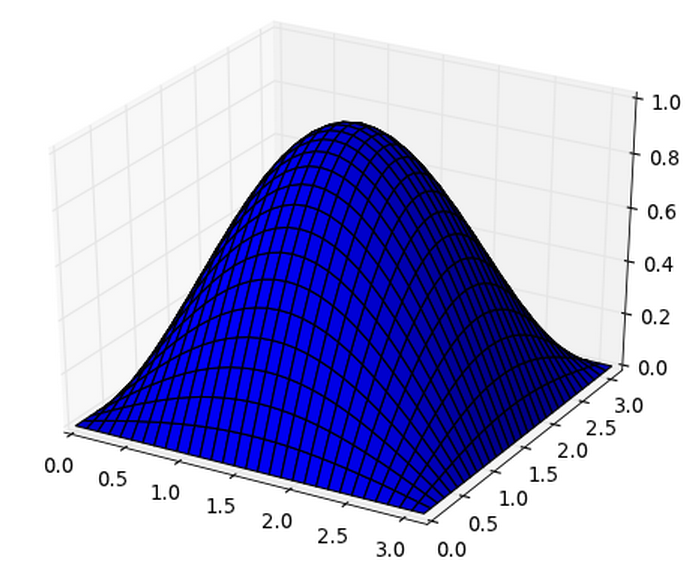
\includegraphics[height=0.5\textwidth]{img/area-1.png}
\end{center}
\noindent
This task 
may seem difficult but we can use similar trick as in Exercises 05.03 and 05.04: Split the rectangle 
(x1, x2)x(y1, y2) into nx times ny equally-sized small rectangles. Moreover, split each of these small rectangles 
diagonally into two triangles (there are two diagonals but it does not matter which one you choose). Over each 
triangle, span a linear plane that in the corners coincides with the function f(x, y). Use the function from Exercise 
05.05 to calculate the triangle area. After adding the area of 
all these triangles together, you will have an approximation of the roof surface. Return it as a result of the function. 
Similarly to Exercises 05.03 and 05.04, experiment with various values of nx and 
ny until you are confident that the surface that you 
calculated is exact to two decimal digits! Test your program on the function f(x, y) = sin(x)*sin(y) in the interval
(0, Pi)x(0, Pi) that is shown below.

%%%%%%%%%%%%%%%%%%%%%%%%%%%%%%%%%%%%%%%%%%%%%%%%%%%%%%%%%%%%%%%%%%%%%%%%%%%%
%%%%%%%%%%%%%%%%%%%%%%%%%%%%%%%%%%%%%%%%%%%%%%%%%%%%%%%%%%%%%%%%%%%%%%%%%%%%

\section{Logic and probability}

In this section we practice usage of logical operations and useful operations 
with random numbers.

%%%%%%%%%%%%%%%%%%%%%%%%%%%%%%%%%%%%%%%%%%%%%%%%%%%%%%%%%%%%%%%%%%%%%%%%%%%%

\subsection{Even or odd}

Write a Python function {\tt checknumber(n)} where {\tt n} is an arbitrary 
integer number, that returns {\tt True} if {\tt n} is even and {\tt False}
otherwise.

%%%%%%%%%%%%%%%%%%%%%%%%%%%%%%%%%%%%%%%%%%%%%%%%%%%%%%%%%%%%%%%%%%%%%%%%%%%%

\subsection{Mysterious parabola}

Consider a quadratic equation $ax^2 + bx + c = 0$ where $a, b, c$ are real numbers 
and $a \not = 0$. Write a Python function 
{\tt hasrealroots(a, b, c)} that returns {\tt True} if the equation has 
at least one real root, and {\tt False} otherwise.

%%%%%%%%%%%%%%%%%%%%%%%%%%%%%%%%%%%%%%%%%%%%%%%%%%%%%%%%%%%%%%%%%%%%%%%%%%%%

\subsection{Point in circle}

Write a Python function {\tt liesincircle(R, x, y)} that returns {\tt True} if 
the point with planar coordinates {\tt [x, y]} lies in a circle of radius {\tt R}
whose center is at the origin {\tt [0, 0]}. If the point lies on the border of the 
circle or outside, the function should return {\tt False}.

%%%%%%%%%%%%%%%%%%%%%%%%%%%%%%%%%%%%%%%%%%%%%%%%%%%%%%%%%%%%%%%%%%%%%%%%%%%%

\subsection{Slot machine}

Write a Python function {\tt slotmachine()} that simulates a simple slot machine
by returning three random integers between 0 and 9. Use the function 
{\tt random()} from the {\tt random} library that returns a random 
real number between 0.0 and 1.0. Hint: Split the interval (0, 1) into 10 
equally-long parts. Return 0 if the generated random number falls into the 
first one, 1 if it falls into the second one, etc. Integer part of a real number
{\tt x} is obtained via {\tt int(x)}.

%%%%%%%%%%%%%%%%%%%%%%%%%%%%%%%%%%%%%%%%%%%%%%%%%%%%%%%%%%%%%%%%%%%%%%%%%%%%

\subsection{Dice game}

Write a Python function {\tt dicegame()} that simulates a throw of two
dice by returning a pair of random numbers 1 - 6. Make sure that 
every number has the same probablity. Use the function 
{\tt random()} from the {\tt random} library that returns a random 
real number between 0.0 and 1.0. Hint: Split the interval (0, 1) into six 
equally-long parts. Return 1 if the generated random number falls into the first one, 
etc. Integer part of a real number {\tt x} is obtained via {\tt int(x)}.

%%%%%%%%%%%%%%%%%%%%%%%%%%%%%%%%%%%%%%%%%%%%%%%%%%%%%%%%%%%%%%%%%%%%%%%%%%%%

\subsection{Cheat dice}

Write a Python function {\tt cheatdice(p1, p2, p3, p4, p5, p6)} that simulates 
a throw of two dice by returning a pair of random numbers 1 - 6. However, this time,
you are using artificially altered dice where the probability of obtaining 1 is p1 
instead of 1/6, probability of obtaining 2 is p2 instead of 1/6, etc. The sum
of all p1, p2, ..., p6 equals to 1.0.
Again use the function {\tt random()} from the {\tt random} library. 
Hint: Split the interval
(0, 1) into six parts which now will not be equally-long. Their lengths will
be p1, p2, ..., p6. If the generated random number falls into the first one, return 1, 
etc.

%%%%%%%%%%%%%%%%%%%%%%%%%%%%%%%%%%%%%%%%%%%%%%%%%%%%%%%%%%%%%%%%%%%%%%%%%%%%

\subsection{Monte Carlo pie}

Probabilistic methods are often called {\em Monte Carlo methods}. 
Write a Python function {\tt calculate\_pi(n)} that will calculate and return 
an approximation of $\pi$ using the following algorithm: Generate $n$ random points 
inside the square $(-1, 1)\times(-1, 1)$. Count the number $m$ of points that 
lie in the circle or radius $r = 1$ centered at the origin, as shown in the 
figure below.

\begin{center}
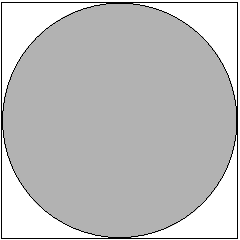
\includegraphics[height=0.3\textwidth]{img/prob1.pdf}
\end{center}
\noindent
Clearly the ratio of 
$m$ and $n$ is approximately the same as the ratio of the area $C$ of the circle 
to the area $S$ of the square. 

$$
\frac{m}{n} \approx \frac{C}{S}
$$
At least for large values of $n$ such as 10,000 this will be close. 
Assume that the number $\pi$ satisfies $C = \pi r^2$. Knowing that $S = 4$, 
we can calculate

$$
\frac{m}{n} \approx \frac{\pi}{4}
$$ 
and thus 

$$
\frac{4m}{n} \approx \pi.
$$ 
Hence, use the last formula to calculate an approximation of $\pi$ using 
the numbers $n$ and $m$.

%%%%%%%%%%%%%%%%%%%%%%%%%%%%%%%%%%%%%%%%%%%%%%%%%%%%%%%%%%%%%%%%%%%%%%%%%%%%

\subsection{Maximum of a function}\label{exe:maximum}

Write a Python function {\tt maxfun(f, a, b, n)} to calculate and return  
an approximate maximum of the function $f(x)$ in the interval $(a, b)$. Hint:
Cover the interval $(a, b)$ with $n$ equidistant points. Loop over the 
points, evaluate the function $f$ at every one of them, and find the maximum 
value.

%%%%%%%%%%%%%%%%%%%%%%%%%%%%%%%%%%%%%%%%%%%%%%%%%%%%%%%%%%%%%%%%%%%%%%%%%%%%

\subsection{Monte Carlo area}

Write a Python function {\tt area\_under\_graph(f, a, b, max, n)} to calculate and return  
an approximation of the area under the graph of the function $f(x)$ in the interval $(a, b)$. By the area
under a graph we understand the area between the $x$-axis and the 
graph in the interval $(a, b)$ as illustrated in the figure below. 

\begin{center}
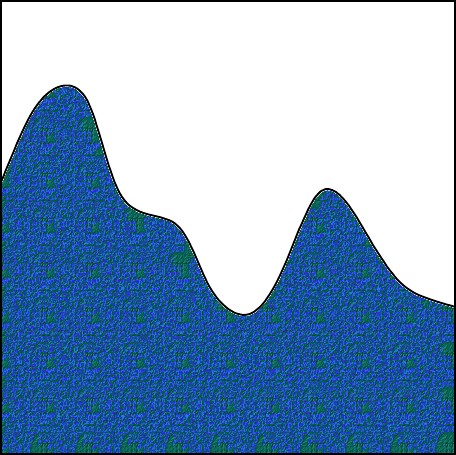
\includegraphics[height=0.3\textwidth]{img/prob2.png}
\end{center}
\noindent
Hint: Use the function {\tt maximum(f, a, b, n)} from Exercise \ref{exe:maximum}
to find an approximate maximum $M$ of the function $f$ in the interval $(a,b)$. 
Generate $n^2$ random points in the rectangle $(a, b)\times(0, M)$. By $m$ denote 
the number of points which lie under the function graph. Clearly, for larger
$n^2$ such as $10000$ the ratio of $m$ and $n^2$ will be approximately the same as 
the ratio of the area $A$ under the graph and the area $R$ of the rectangle $(a, b)\times(0, M)$. 
Hence we obtain 
$$
\frac{m}{n^2} \approx \frac{A}{R}.
$$
From here, it is easy to express $A$ as
$$
A \approx \frac{Rm}{n^2}
$$

%%%%%%%%%%%%%%%%%%%%%%%%%%%%%%%%%%%%%%%%%%%%%%%%%%%%%%%%%%%%%%%%%%%%%%%%%%%%

\subsection{Trapezoids}\label{exe:trap}

Write a Python function {\tt trapezoids(f, a, b, n)} to calculate and return  
an approximate area under the graph of the function $f(x)$ in the interval $(a, b)$. 
First split the interval $(a, b)$ into $n$
equally-long parts, and then add together the areas of all trapezoids under the 
graph of the function $f$, as shown in the image below. 

\begin{center}
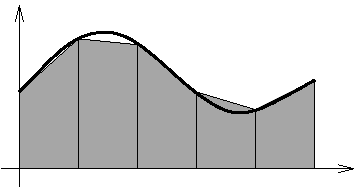
\includegraphics[height=0.3\textwidth]{img/riem.pdf}
\end{center}
\noindent
You can notice that in some cases the entire trapezoid does not lie 
under the curve, but this is OK. It is important that the upper two vertices 
of each trapezoid always lie on the function graph.
Hint: The area of a trapezoid with basis $(c, d)$ and function 
values $f(c),\, f(d)$ at the upper vertices is 
$$
area = (d - c)\frac{f(c) + f(d)}{2}.
$$
Test your code with the function $f(x) = \sin(x)$ in the interval $(0, \pi)$.
In this case the exact area under the graph is $area = 2$.

%%%%%%%%%%%%%%%%%%%%%%%%%%%%%%%%%%%%%%%%%%%%%%%%%%%%%%%%%%%%%%%%%%%%%%%%%%%%
%%%%%%%%%%%%%%%%%%%%%%%%%%%%%%%%%%%%%%%%%%%%%%%%%%%%%%%%%%%%%%%%%%%%%%%%%%%%

\section{Conditional Loop}

In this section we solve problems that include iterations (repetitions) whose
number is not known in advance.

%%%%%%%%%%%%%%%%%%%%%%%%%%%%%%%%%%%%%%%%%%%%%%%%%%%%%%%%%%%%%%%%%%%%%%%%%%%%

\subsection{Water jar}

There is a jar of volume $V$ that is full of water. Every day, 
$P$ per cent of the water volume evaporates. Write a function 
{\tt waterjar(V, P, R)} that prints the remaining water volume day
by day. The process stops when the volume is less than or equal to 
a residual volume $R$. Your function should return the number of 
days the process took. Include a condition at the beginning 
of the function that will output a warning and return zero 
if $R > V$ or $V <= 0$ or $R <= 0$.

%%%%%%%%%%%%%%%%%%%%%%%%%%%%%%%%%%%%%%%%%%%%%%%%%%%%%%%%%%%%%%%%%%%%%%%%%%%%

\subsection{Throwing stones}

Imagine that you stand on a very high bridge $H$ meters above 
a river and throw a stone with velocity $v$ in horizontal direction. 
The coordinates of the flying stone as functions of time $t$ are
$x(t) = t v$ and $y(t) = H - 0.5gt^2$ where $g = 9.81$ kgms$^{-2}$ is
the gravitational acceleration. Use these formulas to write a function 
{\tt flyingstone(t, H, v)} that for any time instant {\tt t} returns the $x$ and 
$y$ coordinates of the flying stone. Then calculate and plot the trajectory 
of the stone since the moment it leaves your hand until it falls into the 
river! Hint: Proceed by choosing a small time step {\tt dt} such 
as $0.01$ seconds, and use the function {\tt flyingstone(t, H, v)} to generate 
a sequence of points for the {\tt plot()} command.  

%%%%%%%%%%%%%%%%%%%%%%%%%%%%%%%%%%%%%%%%%%%%%%%%%%%%%%%%%%%%%%%%%%%%%%%%%%%%

\subsection{Missing numbers}

Write a function {\tt missing\_numbers()} that defines a variable $e = 1.0$ 
and performs a loop in which the value of $e$ is divided by $10.0$. The loop should
run while $1.0 - e < 1.0$. Count how many times the loop will run and return 
this number. Note: Since $1.0 - e$ is no longer less than $1.0$ in the 
computer arithmetic, this clearly shows that the computer arithmetic
does not contain all real numbers!

%%%%%%%%%%%%%%%%%%%%%%%%%%%%%%%%%%%%%%%%%%%%%%%%%%%%%%%%%%%%%%%%%%%%%%%%%%%%

\subsection{Trapezoids revisited}

In this exercise we will reuse the function {\tt trapezoids(f, a, b, n)}
from Exercise \ref{exe:trap}. Write a function {\tt accurate\_area(f, a, b, err)}
that begins with approximationg the area  using just one trapezoid: 
{\tt trapezoids(f, a, b, 1)}. Then write a loop in which the number 
$n$ is doubled and new approximation of the area is calculated. The loop should 
run while the absolute value of the difference between the last two approximations 
is greater than $err$. Return two values: the last (most accurate) area approximation, 
and the number of trapezoids used. Test your function on $f(x) = \exp(-x)$
in the interval $(0, 100)$ and $err = 10^{-8}$. (The exact area in this case is $area = 1$.)

%%%%%%%%%%%%%%%%%%%%%%%%%%%%%%%%%%%%%%%%%%%%%%%%%%%%%%%%%%%%%%%%%%%%%%%%%%%%

\subsection{Infinite sum}

It is a well known fact in mathematics that the sum of the infinite sequence 
$$
\frac{1}{1} + \frac{1}{2^2} +\frac{1}{3^2} + \frac{1}{4^2} + \ldots
$$
is a finite number. But what is this number? Let's find out!
Write a Python function {\tt sum(err)} that will keep adding the 
numbers in the above sequence together until the last increment 
is less than {\tt err}. Then stop, and return two values: the latest 
value of the sum and the number of entries added.

%%%%%%%%%%%%%%%%%%%%%%%%%%%%%%%%%%%%%%%%%%%%%%%%%%%%%%%%%%%%%%%%%%%%%%%%%%%%
%%%%%%%%%%%%%%%%%%%%%%%%%%%%%%%%%%%%%%%%%%%%%%%%%%%%%%%%%%%%%%%%%%%%%%%%%%%%

\section{Strings}

In this section we will practice operations with text strings.

%%%%%%%%%%%%%%%%%%%%%%%%%%%%%%%%%%%%%%%%%%%%%%%%%%%%%%%%%%%%%%%%%%%%%%%%%%%%

\subsection{Spelling}

Write a function {\tt spell(str)} that prints the string {\tt str} one character 
per line, and returns the number of characters in the string.

%%%%%%%%%%%%%%%%%%%%%%%%%%%%%%%%%%%%%%%%%%%%%%%%%%%%%%%%%%%%%%%%%%%%%%%%%%%%

\subsection{Inserting spaces}

Write a function {\tt insert\_spaces(str)} that returns a new string that is obtained 
by inserting an empty character between all letters in {\tt str}. 

%%%%%%%%%%%%%%%%%%%%%%%%%%%%%%%%%%%%%%%%%%%%%%%%%%%%%%%%%%%%%%%%%%%%%%%%%%%%

\subsection{Counting chars}

Write a function {\tt countchars(str, L)} that counts 
all occurrences of the character (one-letter string) {\tt L} in the string {\tt str}, 
and return their number. 

%%%%%%%%%%%%%%%%%%%%%%%%%%%%%%%%%%%%%%%%%%%%%%%%%%%%%%%%%%%%%%%%%%%%%%%%%%%%

\subsection{Counting words}

Write a function {\tt countwords(str, word)} that will count 
all occurences of the string {\tt word} in the string {\tt str}, and 
return their number. You can assume that {\tt len(str)} is always greater 
or equal to {\tt len(word)}.

%%%%%%%%%%%%%%%%%%%%%%%%%%%%%%%%%%%%%%%%%%%%%%%%%%%%%%%%%%%%%%%%%%%%%%%%%%%%

\subsection{Search and replace}

Write a function {\tt searchandreplace(str, word1, word2)} that will 
find all occurrences of the string {\tt word1} in the string {\tt str}, and 
replace them with the string {\tt word2}. Return the new string and the number
of replacements made..
Hint: Do not change the string {\tt str} - instead, 
create a new string {\tt str2} and add into it what is needed.

%%%%%%%%%%%%%%%%%%%%%%%%%%%%%%%%%%%%%%%%%%%%%%%%%%%%%%%%%%%%%%%%%%%%%%%%%%%%
%%%%%%%%%%%%%%%%%%%%%%%%%%%%%%%%%%%%%%%%%%%%%%%%%%%%%%%%%%%%%%%%%%%%%%%%%%%%

\section{Tuples, Lists, and Dictionaries}

In this section we will solve problems related to tuples, lists and dictionaries. 

%%%%%%%%%%%%%%%%%%%%%%%%%%%%%%%%%%%%%%%%%%%%%%%%%%%%%%%%%%%%%%%%%%%%%%%%%%%%

\subsection{List reverse}

Write a Python function {\tt listreverse(L)} that reverts the list {\tt L} and 
returns the result. Use of the Python built-in list reverse function is not allowed. 

%%%%%%%%%%%%%%%%%%%%%%%%%%%%%%%%%%%%%%%%%%%%%%%%%%%%%%%%%%%%%%%%%%%%%%%%%%%%

\subsection{String to list}

Write a Python function {\tt str2list(str)} that for any text string {\tt str} 
returns the list of words that it contains, in the order they appear. Repetitions 
are allowed. Words can be separated by empty character  ' ', comma, period, 
question mark or exclamation mark.

%%%%%%%%%%%%%%%%%%%%%%%%%%%%%%%%%%%%%%%%%%%%%%%%%%%%%%%%%%%%%%%%%%%%%%%%%%%%
%%%%%%%%%%%%%%%%%%%%%%%%%%%%%%%%%%%%%%%%%%%%%%%%%%%%%%%%%%%%%%%%%%%%%%%%%%%%

\section{More on Counting Loop} 

In this section we strengthen our understanding of the counting 
loop by solving problems that include repetitions whose number 
is known in advance.

%%%%%%%%%%%%%%%%%%%%%%%%%%%%%%%%%%%%%%%%%%%%%%%%%%%%%%%%%%%%%%%%%%%%%%%%%%%%

\subsection{Analyze string}

Write a Python function {\tt analyze\_string(str)} that for the text string {\tt str}
returns the number of decimals '0' - '9'. 

%%%%%%%%%%%%%%%%%%%%%%%%%%%%%%%%%%%%%%%%%%%%%%%%%%%%%%%%%%%%%%%%%%%%%%%%%%%%

\subsection{Multiplication table}

Write a Python function {\tt multable(N)} that returns a 2D array 
A containing the multiplicative table of the numbers $1, 2, \ldots, N$. 
In other words, $A[i-1][j-1] = ij$ for all $i, j = 1, 2, ..., N$. Hint: Use 
the Numpy command {\tt zeros} to create the 2D array:

\begin{Verbatim}[commandchars=\\\{\}]
\PY{k+kn}{from} \PY{n+nn}{numpy} \PY{k+kn}{import} \PY{n}{zeros}
\PY{n}{A = zeros}\PY{p}{(}\PY{p}{(}\PY{n}{N}\PY{p}{,} \PY{n}{N}\PY{p}{)}\PY{p}{)}
\end{Verbatim}
Entry at position {\tt r}, {\tt s} in A is accessed via {\tt A[r][s]}. Keep in mind that
indices start from zero. 
 
%%%%%%%%%%%%%%%%%%%%%%%%%%%%%%%%%%%%%%%%%%%%%%%%%%%%%%%%%%%%%%%%%%%%%%%%%%%%

\subsection{Approximating $\pi$}

The number $\pi$ can be written as an infinite series 
$$
\pi = 4\left(1 - \frac{1}{3} + \frac{1}{5} - \frac{1}{7} + \frac{1}{9} - \ldots     \right).
$$
Write a Python function {\tt approx\_pi(n)} that returns an approximation 
of $\pi$ using a truncated series with $n$ terms.

%%%%%%%%%%%%%%%%%%%%%%%%%%%%%%%%%%%%%%%%%%%%%%%%%%%%%%%%%%%%%%%%%%%%%%%%%%%%

\subsection{Prime numbers}

Write a Python function {\tt primes(n)} that for a positive number {\tt n} returns the list 
of first {\tt n} prime numbers starting with 2. 

%%%%%%%%%%%%%%%%%%%%%%%%%%%%%%%%%%%%%%%%%%%%%%%%%%%%%%%%%%%%%%%%%%%%%%%%%%%%

\subsection{List maximizer}

Write a Python function {\tt maximizer(L1, L2)} that takes two lists of real numbers and 
finds a number {\tt n1} in {\tt L1} and a number {\tt n2} in {\tt L2} such that the product 
of {\tt n1} and {\tt n2} is maximal. Return the numbers {\tt n1} and {\tt n2}.

%%%%%%%%%%%%%%%%%%%%%%%%%%%%%%%%%%%%%%%%%%%%%%%%%%%%%%%%%%%%%%%%%%%%%%%%%%%%

\subsection{Fibonacci}

Write a Python function {\tt fibonacci(n)} that returns a list of integer numbers representing 
the Fibonacci sequence. Recall that this sequence starts with 0, 1 and each next number is the 
sum of the two last numbers in the sequence. 

%%%%%%%%%%%%%%%%%%%%%%%%%%%%%%%%%%%%%%%%%%%%%%%%%%%%%%%%%%%%%%%%%%%%%%%%%%%%

\subsection{Adding fractions}

Write a Python function {\tt addfractions(L)} where L is a list of integer pairs (two-element lists). Each integer pair represents the numerator and denominator of a fraction. Your function should add all these fractions together and obtain the numerator and denominator of the resulting fraction. Further, the numerator and denominator should be divided by the greatest common divisor to reduce the fraction to the simplest possible form. Hint: The function fraction.gcd(numerator, denominator) can be used to find the greatest common divisor of two integers.

%%%%%%%%%%%%%%%%%%%%%%%%%%%%%%%%%%%%%%%%%%%%%%%%%%%%%%%%%%%%%%%%%%%%%%%%%%%%
%%%%%%%%%%%%%%%%%%%%%%%%%%%%%%%%%%%%%%%%%%%%%%%%%%%%%%%%%%%%%%%%%%%%%%%%%%%%

\section{Exceptions}

In this section we put exceptions handling to practical use.

%%%%%%%%%%%%%%%%%%%%%%%%%%%%%%%%%%%%%%%%%%%%%%%%%%%%%%%%%%%%%%%%%%%%%%%%%%%%

\subsection{Sure plot}

Implement a custom function {\tt sureplot(f, a, b, label, n = 100)} where {\tt f(x)} is a user-supplied real function, 
$(a, b)$ is an interval, 'label' is a text string label for the plot, and $n$ is the plotting subdivision of the interval $(a, b)$. 
Implement exception handling in such a way that if the user's function is not defined for some $x$, a warning is printed and the 
corresponding point is not added to the plot. But the rest of the graph will be plotted normally. For example, if the user wants 
to plot the function log(x) in the interval (-1, 1) then the left half of the graph will be missing but the rest will be displayed correctly.
\begin{Verbatim}[commandchars=\\\{\}]
\PY{k}{def} \PY{n+nf}{f}\PY{p}{(}\PY{n}{x}\PY{p}{)}\PY{p}{:}
    \PY{k}{return} \PY{n}{log}\PY{p}{(}\PY{n}{x}\PY{p}{)}
\end{Verbatim}
in the interval {\tt (-1, 1)} then the left half of the graph should be missing but the rest 
will be displayed correctly. Hint: Use mathematical functions from the "math" module ("from math 
import log").

%%%%%%%%%%%%%%%%%%%%%%%%%%%%%%%%%%%%%%%%%%%%%%%%%%%%%%%%%%%%%%%%%%%%%%%%%%%%

\subsection{Syntax check}

Implement a Boolean function {\tt syntaxcheck(str)} that evaluates any user-supplied text expression {\tt str}. If the code in {\tt str} contains a syntax error, return False. Otherwise return True. Hint: Text string {\tt str} can be evaluated in Python via the command {\tt exec(str, {})}. Do not worry about the second argument - it serves for passing data into the evaluated expression. Check Python tutorial for more details if interested.

%%%%%%%%%%%%%%%%%%%%%%%%%%%%%%%%%%%%%%%%%%%%%%%%%%%%%%%%%%%%%%%%%%%%%%%%%%%%
%%%%%%%%%%%%%%%%%%%%%%%%%%%%%%%%%%%%%%%%%%%%%%%%%%%%%%%%%%%%%%%%%%%%%%%%%%%%

\section{Object-Oriented Programming}

In this section we practise our understanding of object-oriented programming.

%%%%%%%%%%%%%%%%%%%%%%%%%%%%%%%%%%%%%%%%%%%%%%%%%%%%%%%%%%%%%%%%%%%%%%%%%%%%

\subsection{Bank account}

Implement a Python class {\tt Account} to simulate a bank account. It 
should have two variables {\tt savings} and {\tt checking}, and the following methods:
\begin{itemize}
\item Constructor {\tt \_\_init\_\_(self)} that creates an empty checking and savings account.
\item {\tt add\_to\_checking(self, amount)}: Add {\tt amount} to checking.
\item {\tt add\_to\_savings(self, amount)}: Add {\tt amount} to savings.
\item {\tt get\_balance\_checking(self)}: Return the balance in the checking account.
\item {\tt get\_balance\_savings(self)}: Return the balance in the savings account.
\item {\tt transfer\_to\_checking(self, amount)}: Transfer {\tt amount} from savings to checking
      and return True.
      If there are insufficient funds, do not perform the operation, write a warning,
      and return False. 
\item {\tt transfer\_to\_savings(self, amount)}: Transfer {\tt amount} from checking to savings
      and return True.
      If there are insufficient funds, do not perform the operation, write a warning,
      and return False. 
\item {\tt withdraw\_from\_checking(self, amount)}: Withdraw {\tt amount} from checking
      and return True.
      If there are insufficient funds, do not perform the operation, write a warning,
      and return False. 
\item {\tt withdraw\_from\_savings(self, amount)}: Withdraw {\tt amount} from savings
      and return True.
      If there are insufficient funds, do not perform the operation, write a warning,
      and return False. 

\end{itemize}

%%%%%%%%%%%%%%%%%%%%%%%%%%%%%%%%%%%%%%%%%%%%%%%%%%%%%%%%%%%%%%%%%%%%%%%%%%%%

\subsection{Word magic}

Implement a Python-dictionary-based smart translator class {\tt Wordmagic} that 
will have the following methods:
\begin{itemize}
\item Constructor {\tt \_\_init\_\_(self)} that creates an empty dictionary.
\item {\tt add(self, word, tran)}: Boolean method that adds a pair of text strings into 
      the dictionary. The former is the key, the latter the corresponding value. 
      If {\tt word} is already present in the dictionary,
      let the user know via a warning message, do not add it, and return {\tt False}. 
      Otherwise return {\tt True}.
\item {\tt read(self, d)}: Method that imports existing dictionary.
\item {\tt translate(self, word)}: Method that returns a Boolean and a string. If {\tt word}   
      is present in the keys, return True and its translation. Otherwise print a warning,
      and return False and an empty string.
\item {\tt export(self)}: Method that returns the dictionary.
\item {\tt reverse(self)}: Method that swaps all keys and values in the dictionary.
\end{itemize}

%%%%%%%%%%%%%%%%%%%%%%%%%%%%%%%%%%%%%%%%%%%%%%%%%%%%%%%%%%%%%%%%%%%%%%%%%%%%

\subsection{Number magic}\label{numbermagic}

Implement a Python class {\tt Numbermagic} whose data is just one integer number, and 
whose methods are as follows:
\begin{itemize}
\item Constructor {\tt \_\_init\_\_(self, num)} that takes one integer number as parameter and stores it in the object. 
      If the user supplies a non-integer number, print a warning and round it to an integer.
      Hint: Use Python bbuilt-in function {\tt isinstance(n, int)} to determine whether 
      the number 'n' is integer.
\item {\tt insert(self, num)}: Method that replaces the number stored in the object with {\tt num}.
      As in constructor, make sure that the number is an integer.
\item {\tt ispositive(self)}: Boolean method that returns {\tt True} if the number stored in the object is 
      greater than zero, {\tt False} otherwise.
\item {\tt iseven(self)}: Boolean method that returns {\tt True} if the number stored in the object is even,
      {\tt False} otherwise.
\item {\tt isprime(self)}: Boolean method that returns {\tt True} if the number stored in the object is a prime,
      {\tt False} otherwise.
\end{itemize}

%%%%%%%%%%%%%%%%%%%%%%%%%%%%%%%%%%%%%%%%%%%%%%%%%%%%%%%%%%%%%%%%%%%%%%%%%%%%

\subsection{Vector magic} \label{vectormagic}

Implement a Python class {\tt Vectormagic} whose data are two three-dimensional vectors.
All vectors are represented by lists of length three. The class has the following methods:
\begin{itemize}
\item Constructor {\tt \_\_init\_\_(self, u, v)} that takes two vectors as parameters and stores them in the object. 
      If the length of any of the two vectors is not three, raise a ValueError exception.
\item {\tt insert(self, u, v)}: Method that replaces the vectors in the object with new ones.
      Make sure that u, v are 3D vectors same as in the constructor.
\item {\tt norm(self, z)}: Method to calculate the Euclidean norm of vector {\tt z}.
\item {\tt areparallel(self)}: Boolean method that returns {\tt True} if the vectors are parallel,
      {\tt False} otherwise. Note: If you are going to compare a real number against zero,
      use a small tolerance, such as {\tt 1e-8}.
\item {\tt arenormal(self)}: Boolean method that returns {\tt True} if the vectors are perpendicular,
      {\tt False} otherwise. Again: If you are going to compare a real number against zero,
      use a small tolerance, such as {\tt 1e-8}.
\item {\tt innerproduct(self)}: Returns one real number which is the inner product of the two vectors.
\item {\tt vectorproduct(self)}: Returns a vector (list of length three) which is the vector product 
      of the two vectors.
\end{itemize}

%%%%%%%%%%%%%%%%%%%%%%%%%%%%%%%%%%%%%%%%%%%%%%%%%%%%%%%%%%%%%%%%%%%%%%%%%%%%
%%%%%%%%%%%%%%%%%%%%%%%%%%%%%%%%%%%%%%%%%%%%%%%%%%%%%%%%%%%%%%%%%%%%%%%%%%%%

\section{Class Inheritance}

In this section we solve problems involving creating descendants of classes 
in object-oriented programming. 

%%%%%%%%%%%%%%%%%%%%%%%%%%%%%%%%%%%%%%%%%%%%%%%%%%%%%%%%%%%%%%%%%%%%%%%%%%%%

\subsection{Number master}

Create a descendant {\tt Numbermaster} of the class {\tt Numbermagic} from Exercise \ref{numbermagic}
that in addition to the functionality contained in the class {\tt Numbermagic} has one new
method:
\begin{itemize}
\item {\tt factorize(self)}: Method that returns a Python list containing primes {\tt p1, p2, ..., pn}
      that form the prime number factorization of the number stored in the object (repetitions are 
      allowed).
\end{itemize}

%%%%%%%%%%%%%%%%%%%%%%%%%%%%%%%%%%%%%%%%%%%%%%%%%%%%%%%%%%%%%%%%%%%%%%%%%%%%

\subsection{Vector master}

Create a descendant {\tt Vectormaster} of the class {\tt Vectormagic} from Exercise \ref{vectormagic}
that in addition to the functionality contained in the class {\tt Vectormagic} has one new
method:
\begin{itemize}
\item {\tt project(self, w)}: If the two vectors contained in the object form a plane, the 
      method calculates and returns the projection of the vector {\tt w} into this plane. 
      Otherwise the method prints a warning and returns a zero vector. 
\end{itemize}
